\documentclass{article}
\usepackage{amsmath}
\usepackage{graphicx}
\graphicspath{{./images/}}

\begin{document}
\title{Lecture 5: About Images}
\author{Adam Hawley}

\maketitle

\section{Scenes \& Images --- The Basics}
\subsection{Intro}
\begin{itemize}
	\item Images represent a projection of the information from a scene in 2D.
	\item Scenes are real in vision, and created in graphics.
\end{itemize}
\subsection{What is an image?}
\begin{itemize}
	\item An image is a grid of pixels characterised by image size and pixel values.
	\item Each grey-level image pixel has 8 bits so its value ranges from 0--255. 
	\item Each colour pixel has 3 colour components: red, green and blue.
\end{itemize}

\subsection{Histograms}
Histograms represent the {\it the global statistical information} from the image, which may or may not correspond to a specific object. 
They count the frequency of each value in the image.

Histograms are represented as 1-D arrays for grey-level images and as 3-D arrays for colour images - one for each component.

Histogram stretching represents a mapping of the histogram aiming to improve contrast.

\subsection{Graphical Objects and 3D}
\begin{itemize}
	\item Voxel representaions can be made by adding layers of images together, producing a volumetric (3D) image.
	\item A {\it graphical object} can be represented as a mesh which is a sequence of vertices joined by polygons (usually triangles).
\end{itemize}

\section{Image Production}
\subsection{Abstract View}
Stepping back, one can see that image production has four important properties, the latter two of which will be discussed in greater detail later in the notes.
\begin{enumerate}
	\item Images represent projections of real scenes as viewed by the human eye or as taken by a camera.
	\item Images also represent projections of artificially generated scenes in computer graphics.
	\item The theoretical model of vision we use is called the {\it Pinhole Camera}
	\item The more accurate model of real life is known as the {\it Thin Lens Camera}
\end{enumerate}
\subsection{Pinhole Camera}

\begin{figure}[h]
	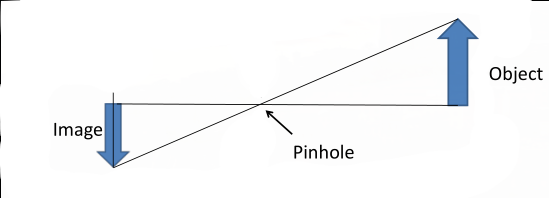
\includegraphics[width=\textwidth]{pinhole.png}
	\label{fig:pinhole}
\end{figure}
The pinhole camera model allows us to use a simplified model of a camera as in figure \ref{fig:pinhole}.
\end{document}
